\section{TCP protocol}
TCP\footnote{Transmission Control Protocol}는 OSI 7계층 중 Transport Layer에서 사용되는 프로토콜로, 
통신과정에서 정보를 안정적으로, 순서대로 에러없이 교환할것을 보장해주는 기능을 수행하는 프로토콜이다.\\
\vspace{-4mm}  
\begin{wrapfigure}{l}{0.5\textwidth} \vspace{-20pt}
\begin{center}
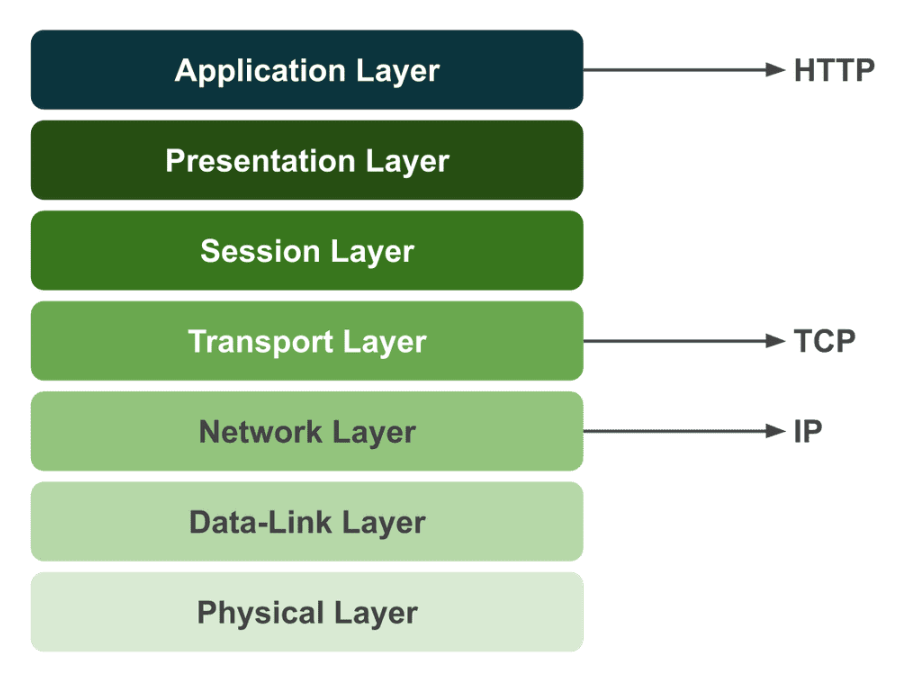
\includegraphics[width=0.43\textwidth]{image/week01/1-0.png}    
\end{center}
\vspace{-20pt}
\caption{\small OSI 7 Layer}
\vspace{-10pt}
\end{wrapfigure}
7계층 구조를 이룸으로서, 네트워크라는 수많은 기술의 집약체에서 각각 계층간의 역할 분담을 통해서 각 작업별로 신경써야 되는 범주 부분을 한정시켜준다. 
예를들어 HTTP 라는 application 요소를 다룰때, 그떄의 DNS 나 packet의 처리 등등의 문제는 별도로 다룰수 있는 점을 들 수 있다. 

Transport Layer로서 데이터의 전송하는 방법은 전송하고자 하는 Data를 Packet으로 나누고 이를 여러 Router를 거처 Destination 까지 전송하는 일련의 과정이고, TCP protocol은 이러한 Packet의 전송에서 완전성을 보장하는 역할을 수행한다. 
TCP packet이 어떻게 완전성을 보장하는지 TCP segment의 Header를 통해 packet의 구성을 확인해 보자.
\subsection{TCP packet의 구성}
    HTTP, TCP, IP와 같은 protocol들은 각 layer에서 고유의 역할을 수행하고, 
    각각 다루는 data들을 layer의 기능에 따라 data에 자신의 \textbf{Header}를 붙이는 방법을 통해서 정보를 표현한다. 
    
    TCP는 packet의 전송에 있어 신뢰성과, 흐름제어, 혼잡제어등의 역할을 수행하는 protocol이기 떄문에, 
    각각의 Header에 기능을 수행하기 위한 값들이 포함되어 있다. \\
    \vspace{-4mm}  
        \begin{figure}[!h]\centering
    		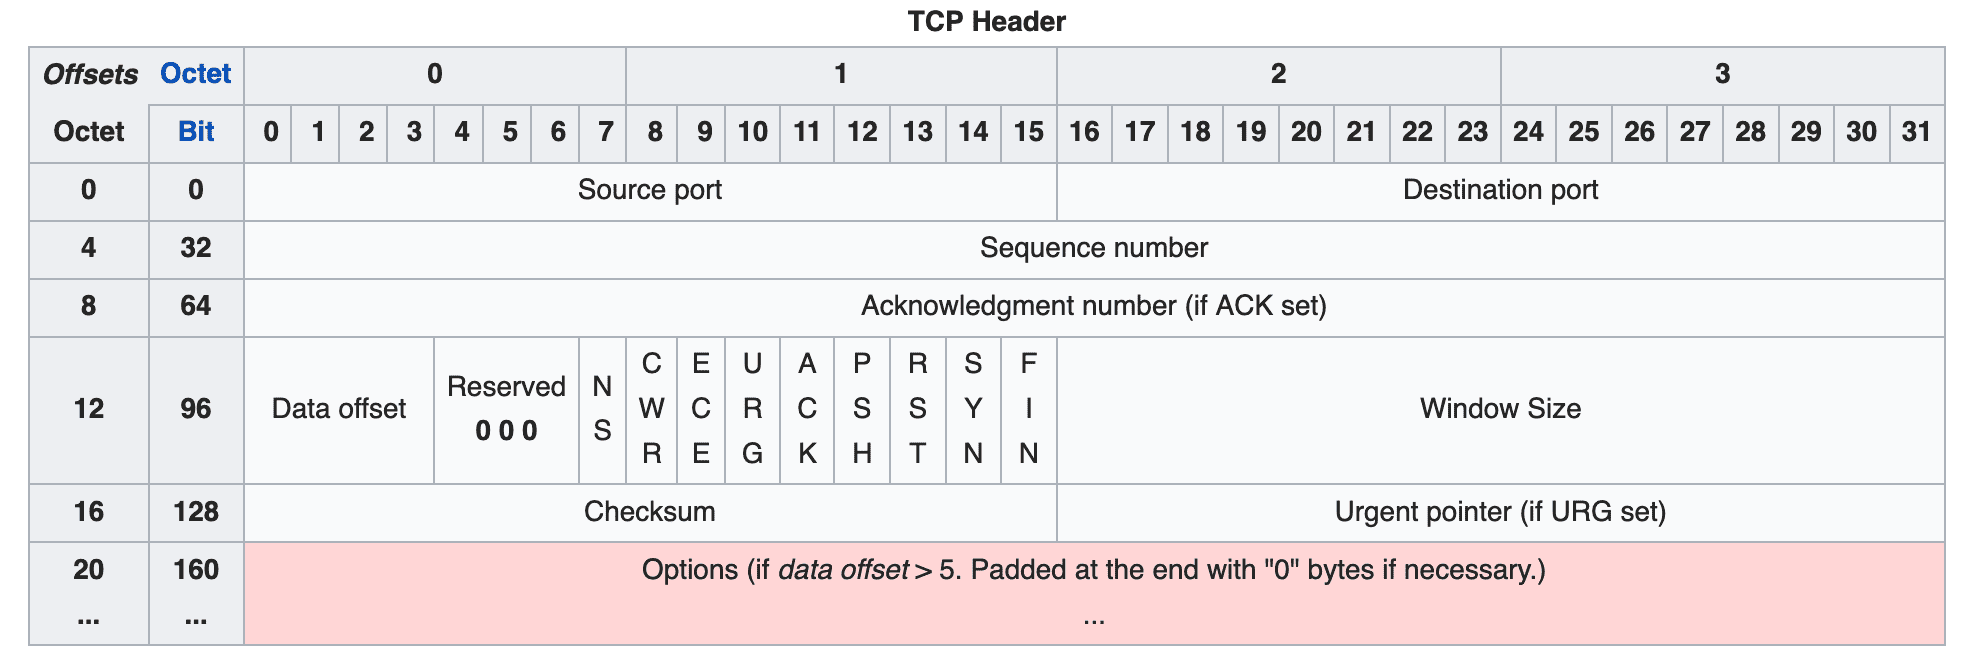
\includegraphics[width=.9\textwidth]{image/week01/1-1-1.png}
    		\caption{\small TCP Header}
    		\label{fig:TCP}
    		\vspace{-10pt}
        \end{figure}

    TCP는 기본적으로 별도로 나누어진 20 Byte, 160 bit의 Binary를 Header로 사용한다.  
    만일 추가의 option field 이용시에 40 Byte, 최대 60 Byte까지 지원이 가능하다. 
\newpage
    \subsubsection*{Source port, Destination port}
        이 필드에서 전송할 segment의 출발지와 목적지를 나타낸다. 
        각각 16 bits로 IP address 와 포트번호 를 통해서 표현한다. 
        Transport Layer에 포함되는 TCP 의 경우 IP 주소는 한 계층 아래인  Network Layer 의 IP header에 담기기 때문에 TCP header에는 IP 주소를 나타내는 필드가 없고 포트번호만을 나타내는 필드만 존재한다.
    \subsubsection*{Sequence Number}
        앞서 TCP의 base가 전송하고자 하는 data를 각각의 packet으로 나누어 전송하는것이고, 
        sequence number를 통해서 쪼개진 Segemnent의  순서대로 data를 재조립한다. 
        figure \ref{fig:TCP}에서 확인할 수 있듯이 총 32bits를 할당받고, 이는 4,294,657,296 의 sequence를 담을 수 있음을 의미한다. 
        데이터를 최초로 전송할때 random한 번호로 initialize 시키며, 이후 보내는 데이터의 1 bytes 당 sequence number를 1씩 증가 시킨다.
    \subsubsection*{Acknowledgement Number}
        \vspace{-4mm}  
        \begin{figure}[!h]\centering
    		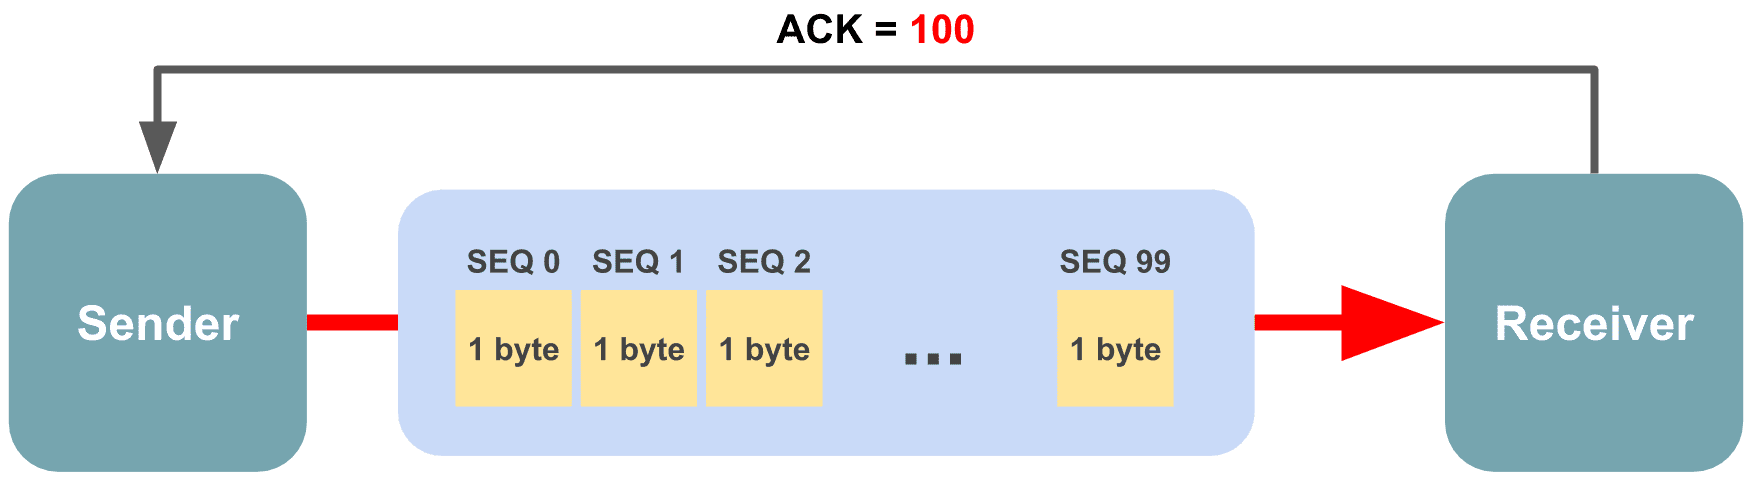
\includegraphics[width=.7\textwidth]{image/week01/1-1-2.png}
    		\caption{\small ACK flow diagram}
    		\vspace{-10pt}
        \end{figure}
    	ACK은 데이터를 받은 수신자가 예상하는 다음 Sequence Number를 의미하고 크기는 Sequence Numer와 동일한 32 bits 이다. 
    	처음 연결을 설정하는 handshake 과정\footnote{이는 Section 1.b 의 SYN segment 와 SYNACK의 Handshake 에서 다루고자 한다. }
    	에서는 “상대방이 보낸 Sequence Number + 1” 로, 데이터를 주고받는 과정에서는 
    	“상대방이 보낸 Sequence Number + 자신이 받은 데이터의 Bytes”로 ACK을 만들어낸다.
    	즉 ACK 은 다음에 보내주어야할 데이터의 시작점을 의미한다. 
    \subsubsection*{Data Offset}\label{sec:data offset}
        Data offset field 는 전체 segment 중에서 Header가 아닌 전송하고자 하는 data가 어디서부터 시작하는지 표기해준다. 
        이는 TCP의 옵션 field 부분의 길이가 사용여부에 따라 가변적이기 때문이다. 
        32 비트 워드를 사용하며, 이떄 32 bit 체계에서는 1 Word = 4 bytes 이다. 
        즉 Data Offset field의 value에 4를 곱해주면 segment에서 header를 제외한 실제 데이터의 시작 위치를  확인할 수 있다.
    \subsubsection*{Reserved (3 bits)}\label{sec:reserved}
        미래를 위해 예약된 필드로, 모두 0 3bit를 채워준다.
    \subsubsection*{Flags (NS ~ FIN)}   
        9개의 비트 플래그이다. 이 플래그들은 현재 세그먼트의 속성을 나타낸다. 
        기존에는 6개의 플래그만을 사용했지만, 혼잡 제어 기능의 향상을 위해 Reserved 필드를 사용하여 NS, CWR, ECE flag가 추가되었다.
        
        우선 기존에 사용되는 6가지 flag의 의미를 table로 정리해 보았다. 추가된 3개의 flag는 네트워크의 
        ECN\footnote{Explict Congestion Notification, 명시적 혼잡통보}를 위해 사용되는 \textbf{NS, CWR, ECE} flag 이다. ECN은 앞서 '000'로 남겨놓은 \nameref{sec:reserved} field의 3 bits를 이용하고,  기존의 Time-Out을 이용한 네트워크 혼잡인지 방법의 비효율성을 개선하기 위해 혼잡상태를 직접 알려주는 방법이다.
        
        ECN은 \textbf{CWR, ECE, ECT, CE} flag들을 이용해서 상대방에서 네트워크의 혼잡도의 정보를 전달할 수 있는데 이중 \textbf{CWR, ECE} 는 Transport Layer인 TCP header에, \textbf{ECT, CE} flag는 Network Layer인 IP header에 존재한다.
\newpage
        \begin{table}[]
        \begin{tabular}{|c|c|}
        \hline
        \multicolumn{1}{|l|}{필드} & \multicolumn{1}{c|}{\textbf{의미}}                                                                                                            \\ \hline
        URG &
          \begin{tabular}[c]{@{}c@{}}Urgent Pointer 필드의 값이 채워져 있음을 알려주는 flag.\\ 포인터가 가르키는 데이터가 우선적으로 처리되나, 50년대 고안된 TCP 성격상 요즘에는 사용되지 않는다.\end{tabular} \\ \hline
        ACK & \begin{tabular}[c]{@{}c@{}}Acknowledgement 필드의 값이 채워져 있음을 알려주는 flag 이 flag가 0 이면 ACK 값이 무시된다.\end{tabular} \\ \hline
        PSH &
          \begin{tabular}[c]{@{}c@{}}Push flag. 수신측에 이 데이터를 최대한 빨리 application에 전달하라는 것을 알려주는 flag.\\ flag가 0이면 수신측은 자신의 buffer가 채워질때 까지 기다린다. 즉 flag가 1이라는 것은 이 segment이후로\\ 연결된 segment가 없다는것을 의미한다.\end{tabular} \\ \hline
        RST & Reset flag.                                                                                                  \\ \hline
        SYN & Synchronize flag. 상대방과 연결을 생성할때 sequence number와 동기화를 위한  segment임을 의미한다.                                    \\ \hline
        FIN & Finish flag                                                                                                  \\ \hline
        \end{tabular}
        \caption{The meaning of 6 classic flags in Flags field in TCP's header}
        \end{table}
        \begin{table}[]
        \begin{tabular}{|c|c|}
        \hline
        \multicolumn{1}{|l|}{필드} & \multicolumn{1}{c|}{\textbf{의미}}                              \\ \hline
        NS                       & ECN 에서 사용하는 CWR, ECE 필드가 실수나 악의적으로 은폐되는것을 대비해 추가된 필드 \\ \hline
        ECE &
          \begin{tabular}[c]{@{}c@{}}ECN Echo flag. 위 필드가 0 이면서, SYN flag가 1일때 ECN을 사용한다고 알리는 의미.\\ 이떄 SYN flag가 0이라는것은 네트워크가 혼잡하기 때문에 segment window 크기를 줄여달라는 의미\end{tabular} \\ \hline
        CWR                      & 이미 ECE로 부터 flag를 받아서 segment의 크기를 줄였다는것을 확인하는 flag   \\ \hline
        \end{tabular}
        \caption{The meaning of 3 flags that used fof ECN in Flags field in TCP's header}
        \end{table}
    \subsubsection*{Window Size}\label{sec: window size}    
        window size field의 값은 한번에 전송할 수 있는 data의 크기의 값을 가진다. 
        $2^{16} = 65535$ 만큼의 값을 표현할 수 있고, 이는 윈도우의 쵀대 크기가 64kb 라는의미이다.
        현대의 통신환경과는 맞지 않는 단위이므로, 비트를 왼쪽으로 shift 하는 방법으로 scale을 키워주는 \textbf{WSCALE} 방법들을
        이용한다. \textbf{WSCALE}을 통해서 얼마나 shift 할지의 값은 option field에 존재한다. 
    \subsubsection*{Check Sum}
        데이터의 송신과정에서 발생할 수 있는 오류를 검출하는 역할을 수행한다. Wraparound를 이용헤 carry를 더해준 값에서 1의 Complement를 취해 Checksum 값을 만들어 준다. 이때의 Wraparound의 값에 송신측에서 보내준 wraparound 의 1의 complement인 cheksum 을 더해줘서 모든 비트가 1이라면 정상적인 것이고, 하나라도 0이 검출될 시에 이는 송신과정에서 오류가 발생했음을 확인할 수 있다.
    \subsubsection*{Urgent Pointer}
        URG flag가 1의값을 가진다면, 수신측은 Urgent Pointer의 adr에 있는 데이터를 우선적으로 처리한다.
    \subsubsection*{Options}
        TCP의 기능을 확장하는데  사용하는 필드이다. 앞서 언급된 \nameref{sec: window size}의 scale을 조절하는 WSCALE , Selective Repeat등을 포함하는 SACK 등이 있으며, 이는 옵션의 포함여부에 따라서 Option의 필드의 크기가 가변적이게 된다. 
        Options field의 길이가 변함에따라 header의 길이 또한 변하게 되고, 이는 수신측에서 어디서부터가 header이고 어디서부터가 data인지 확인하기 위해 offset field를 통해서 이를 전달한다. 
        
        즉 32비트 워드를 사용하는 \nameref{sec:data offset} field의 값을 통해서 이 값의 4를 곱하는 지점에서 실제 헤더를 제외한 데이터가 시작하는 것을 알리는데, \nameref{sec:data offset} field 의 크기가 4 bits 이므로,  최대 $4\ \times\ 2^4 = 60$ bytes 까지 표현할 수 있다. 
        이때 options를 제외한 필수 Header 가 160 bits 즉 20 bytes$\ = 4 \times 5 \text{ (offset's vlaue)}$ 를 차지하므로, TCP header의 size가 20 bytes \~ 60 bytes 사이일때 즉, $\text{data offset} > 5$ 일때 20 bytes 에서 초과한 만큼 Options field에서 0 을 채워주어, 수신측에서 header의 size를 확인할 수 있게 해준다.